
\documentclass[a4paper,12pt]{article}

\usepackage{cmap}

\usepackage[T2A]{fontenc}
\usepackage[utf8x]{inputenc}
\usepackage[russian]{babel}

\usepackage[a4paper,margin=1.5cm,footskip=1cm,left=2cm,right=1.5cm,top=1.5cm
	,bottom=2.0cm]{geometry}
\usepackage{textcase}
\usepackage{csquotes}
\usepackage{enumitem}

\usepackage{ucs}                                              %%
\usepackage{color}                                            %%
\usepackage{array}                                            %%
\usepackage{longtable}                                        %%
\usepackage{calc}                                             %%
\usepackage{multirow}                                         %%
\usepackage{hhline}                                           %%
\usepackage{ifthen}                                           %%
%%  optionally (for landscape tables embedded in another document): %%
\usepackage{lscape}                                           %%

\usepackage{caption}

\usepackage{amsmath}
\usepackage{pgfplots}

\usepackage{float}


\setlist[description]{leftmargin=\parindent,labelindent=\parindent}

\begin{document}

\setcounter{secnumdepth}{0}

\begin{titlepage}

	\begin{center}
		Новосибирский государственный технический университет
		
		Факультет прикладной математики и информатики
		
		Кафедра теоретической и прикладной информатики
		
		\vspace{250pt}
		
		\textbf{\LARGE{Лабораторная работа № 2}}
		\medbreak
		\large{<<Экспериментальное исследование робастности оценок>>}\\
		\medbreak
		по дисциплине\\
		\medbreak
		<<Компьютерные технологии анализа данных и исследования 
			статистических~закономерностей>>
		\vspace{150pt}
	\end{center}

	\begin{flushleft}
		\begin{tabbing}
			Группа:\qquad\qquad	\= ПММ-61\\
			Студент:			\> Горбунов К. К.\\
			Преподаватель:		\> проф. Лемешко Б. Ю.\\
			Вариант:			\> 12 \\
		\end{tabbing}
	\end{flushleft}

	\begin{center}
		\vspace{\fill}
		Новосибирск, 2016 г.
	\end{center}

\end{titlepage}

\newpage

\section{Цель работы}

Исследование устойчивости оценок на наличие в выборке
аномальных наблюдений. Исследование эффективности параметрической
процедуры исключения аномальных наблюдений при использовании робастных
оценок. Построение функций влияния Хампеля для ОМП. Исследование
распределений статистик типа Граббса, предназначенных для анализа на
аномальность сразу нескольких наблюдений.

\section{Краткие теоретические сведения}

\subsection{Модель засорения выборки}

Пусть в эксперименте наблюдается
непрерывная случайная величина $\xi$ с функцией распределения
\[
	F_{\xi}(x) = (1 - \nu) F(x, \theta) + \nu F_1 (x , \theta'),
\]
где $\nu$ - доля засорения выборки аномальными (с точки зрения закона $F(x,
\theta)$) наблюдениями, подчиняющимися закону $F_1(x, \theta_1)$. По выборке
${X_n = \{X_1, X_2, \ldots, X_n\}}$ требуется оценить неизвестные параметры
закона распределения $F(x, \theta)$.

\section{Ход работы}

Вариант 12: \\
$F(x, \theta)$ --- экспоненциальное распределение\\
$F_{1}(x, \theta')$ --- экспоненциальное с масштабом 10


\begin{enumerate}
\item Исследовать робастность оценок максимального правдоподобия (ОМП);
ОМП по группированным данным; MD-оценок, минимизирующих расстояния,
задаваемые статистиками Колмогорова, $\omega^2$ и $\Omega^2$ Мизеса;
$L$-оптимальных оценок по выборочным квантилям. Для этого:
	\begin{itemize}
	\item моделируются выборки с засорением, где параметр $\nu = 0, 0.1, 0.2$;
	\item оцениваются параметры распределения $F(x, \theta)$ всеми методами;
	\item сравниваются значения оценок при разных значениях $\nu$.
	\end{itemize}

Результаты представлены далее в сводной таблице \ref{table:anomest}.

\item Отбраковка аномальных наблюдений. Используя параметрическую
процедуру отбраковки аномальных наблюдений очистить полученные в п.1
выборки от аномальных наблюдений и проверить, как изменились результаты
применения критериев для проверки согласия эмпирического распределения с
распределением $F(x, \theta)$ после удаления части наблюдений.

Результаты представлены в сводной таблице \ref{table:anomest}. 

\def\inputGnumericTable{}
%%%%%%%%%%%%%%%%%%%%%%%%%%%%%%%%%%%%%%%%%%%%%%%%%%%%%%%%%%%%%%%%%%%%%%
%%                                                                  %%
%%  This is the header of a LaTeX2e file exported from Gnumeric.    %%
%%                                                                  %%
%%  This file can be compiled as it stands or included in another   %%
%%  LaTeX document. The table is based on the longtable package so  %%
%%  the longtable options (headers, footers...) can be set in the   %%
%%  preamble section below (see PRAMBLE).                           %%
%%                                                                  %%
%%  To include the file in another, the following two lines must be %%
%%  in the including file:                                          %%
%%        \def\inputGnumericTable{}                                 %%
%%  at the beginning of the file and:                               %%
%%        \input{name-of-this-file.tex}                             %%
%%  where the table is to be placed. Note also that the including   %%
%%  file must use the following packages for the table to be        %%
%%  rendered correctly:                                             %%
%%    \usepackage{ucs}                                              %%
%%    \usepackage[utf8x]{inputenc}                                  %%
%%    \usepackage[T2A]{fontenc}    % if cyrillic is used            %%
%%    \usepackage{color}                                            %%
%%    \usepackage{array}                                            %%
%%    \usepackage{longtable}                                        %%
%%    \usepackage{calc}                                             %%
%%    \usepackage{multirow}                                         %%
%%    \usepackage{hhline}                                           %%
%%    \usepackage{ifthen}                                           %%
%%  optionally (for landscape tables embedded in another document): %%
%%    \usepackage{lscape}                                           %%
%%                                                                  %%
%%%%%%%%%%%%%%%%%%%%%%%%%%%%%%%%%%%%%%%%%%%%%%%%%%%%%%%%%%%%%%%%%%%%%%



%%  This section checks if we are begin input into another file or  %%
%%  the file will be compiled alone. First use a macro taken from   %%
%%  the TeXbook ex 7.7 (suggestion of Han-Wen Nienhuys).            %%
\def\ifundefined#1{\expandafter\ifx\csname#1\endcsname\relax}


%%  Check for the \def token for inputed files. If it is not        %%
%%  defined, the file will be processed as a standalone and the     %%
%%  preamble will be used.                                          %%
\ifundefined{inputGnumericTable}

%%  We must be able to close or not the document at the end.        %%
	\def\gnumericTableEnd{\end{document}}


%%%%%%%%%%%%%%%%%%%%%%%%%%%%%%%%%%%%%%%%%%%%%%%%%%%%%%%%%%%%%%%%%%%%%%
%%                                                                  %%
%%  This is the PREAMBLE. Change these values to get the right      %%
%%  paper size and other niceties.                                  %%
%%                                                                  %%
%%%%%%%%%%%%%%%%%%%%%%%%%%%%%%%%%%%%%%%%%%%%%%%%%%%%%%%%%%%%%%%%%%%%%%

	\documentclass[12pt%
			  ,landscape%
                    ]{report}
       \usepackage{ucs}
       \usepackage[utf8x]{inputenc}
       \usepackage[T2A]{fontenc}
       \usepackage{fullpage}
       \usepackage{color}
       \usepackage{array}
       \usepackage{longtable}
       \usepackage{calc}
       \usepackage{multirow}
       \usepackage{hhline}
       \usepackage{ifthen}

	\begin{document}


%%  End of the preamble for the standalone. The next section is for %%
%%  documents which are included into other LaTeX2e files.          %%
\else

%%  We are not a stand alone document. For a regular table, we will %%
%%  have no preamble and only define the closing to mean nothing.   %%
    \def\gnumericTableEnd{}

%%  If we want landscape mode in an embedded document, comment out  %%
%%  the line above and uncomment the two below. The table will      %%
%%  begin on a new page and run in landscape mode.                  %%
       \def\gnumericTableEnd{\end{landscape}}
       \begin{landscape}


%%  End of the else clause for this file being \input.              %%
\fi

%%%%%%%%%%%%%%%%%%%%%%%%%%%%%%%%%%%%%%%%%%%%%%%%%%%%%%%%%%%%%%%%%%%%%%
%%                                                                  %%
%%  The rest is the gnumeric table, except for the closing          %%
%%  statement. Changes below will alter the table's appearance.     %%
%%                                                                  %%
%%%%%%%%%%%%%%%%%%%%%%%%%%%%%%%%%%%%%%%%%%%%%%%%%%%%%%%%%%%%%%%%%%%%%%

\providecommand{\gnumericmathit}[1]{#1} 
%%  Uncomment the next line if you would like your numbers to be in %%
%%  italics if they are italizised in the gnumeric table.           %%
%\renewcommand{\gnumericmathit}[1]{\mathit{#1}}
\providecommand{\gnumericPB}[1]%
{\let\gnumericTemp=\\#1\let\\=\gnumericTemp\hspace{0pt}}
 \ifundefined{gnumericTableWidthDefined}
        \newlength{\gnumericTableWidth}
        \newlength{\gnumericTableWidthComplete}
        \newlength{\gnumericMultiRowLength}
        \global\def\gnumericTableWidthDefined{}
 \fi
%% The following setting protects this code from babel shorthands.  %%
 \ifthenelse{\isundefined{\languageshorthands}}{}{\languageshorthands{english}}
%%  The default table format retains the relative column widths of  %%
%%  gnumeric. They can easily be changed to c, r or l. In that case %%
%%  you may want to comment out the next line and uncomment the one %%
%%  thereafter                                                      %%
\providecommand\gnumbox{\makebox[0pt]}
%%\providecommand\gnumbox[1][]{\makebox}

%% to adjust positions in multirow situations                       %%
\setlength{\bigstrutjot}{\jot}
\setlength{\extrarowheight}{\doublerulesep}

%%  The \setlongtables command keeps column widths the same across  %%
%%  pages. Simply comment out next line for varying column widths.  %%
\setlongtables

\setlength\gnumericTableWidth{%
	164pt+%
	53pt+%
	44pt+%
	53pt+%
	65pt+%
	53pt+%
	42pt+%
	53pt+%
	65pt+%
0pt}
\def\gumericNumCols{9}
\setlength\gnumericTableWidthComplete{\gnumericTableWidth+%
         \tabcolsep*\gumericNumCols*2+\arrayrulewidth*\gumericNumCols}
\ifthenelse{\lengthtest{\gnumericTableWidthComplete > \linewidth}}%
         {\def\gnumericScale{\ratio{\linewidth-%
                        \tabcolsep*\gumericNumCols*2-%
                        \arrayrulewidth*\gumericNumCols}%
{\gnumericTableWidth}}}%
{\def\gnumericScale{1}}

%%%%%%%%%%%%%%%%%%%%%%%%%%%%%%%%%%%%%%%%%%%%%%%%%%%%%%%%%%%%%%%%%%%%%%
%%                                                                  %%
%% The following are the widths of the various columns. We are      %%
%% defining them here because then they are easier to change.       %%
%% Depending on the cell formats we may use them more than once.    %%
%%                                                                  %%
%%%%%%%%%%%%%%%%%%%%%%%%%%%%%%%%%%%%%%%%%%%%%%%%%%%%%%%%%%%%%%%%%%%%%%

\ifthenelse{\isundefined{\gnumericColA}}{\newlength{\gnumericColA}}{}\settowidth{\gnumericColA}{\begin{tabular}{@{}p{164pt*\gnumericScale}@{}}x\end{tabular}}
\ifthenelse{\isundefined{\gnumericColB}}{\newlength{\gnumericColB}}{}\settowidth{\gnumericColB}{\begin{tabular}{@{}p{53pt*\gnumericScale}@{}}x\end{tabular}}
\ifthenelse{\isundefined{\gnumericColC}}{\newlength{\gnumericColC}}{}\settowidth{\gnumericColC}{\begin{tabular}{@{}p{44pt*\gnumericScale}@{}}x\end{tabular}}
\ifthenelse{\isundefined{\gnumericColD}}{\newlength{\gnumericColD}}{}\settowidth{\gnumericColD}{\begin{tabular}{@{}p{53pt*\gnumericScale}@{}}x\end{tabular}}
\ifthenelse{\isundefined{\gnumericColE}}{\newlength{\gnumericColE}}{}\settowidth{\gnumericColE}{\begin{tabular}{@{}p{65pt*\gnumericScale}@{}}x\end{tabular}}
\ifthenelse{\isundefined{\gnumericColF}}{\newlength{\gnumericColF}}{}\settowidth{\gnumericColF}{\begin{tabular}{@{}p{53pt*\gnumericScale}@{}}x\end{tabular}}
\ifthenelse{\isundefined{\gnumericColG}}{\newlength{\gnumericColG}}{}\settowidth{\gnumericColG}{\begin{tabular}{@{}p{42pt*\gnumericScale}@{}}x\end{tabular}}
\ifthenelse{\isundefined{\gnumericColH}}{\newlength{\gnumericColH}}{}\settowidth{\gnumericColH}{\begin{tabular}{@{}p{53pt*\gnumericScale}@{}}x\end{tabular}}
\ifthenelse{\isundefined{\gnumericColI}}{\newlength{\gnumericColI}}{}\settowidth{\gnumericColI}{\begin{tabular}{@{}p{65pt*\gnumericScale}@{}}x\end{tabular}}

\begin{longtable}[c]{%
	b{\gnumericColA}%
	b{\gnumericColB}%
	b{\gnumericColC}%
	b{\gnumericColD}%
	b{\gnumericColE}%
	b{\gnumericColF}%
	b{\gnumericColG}%
	b{\gnumericColH}%
	b{\gnumericColI}%
	}

%%%%%%%%%%%%%%%%%%%%%%%%%%%%%%%%%%%%%%%%%%%%%%%%%%%%%%%%%%%%%%%%%%%%%%
%%  The longtable options. (Caption, headers... see Goosens, p.124) %%
\captionsetup{justification=raggedleft,singlelinecheck=false}
\caption{}             	%
\label{table:anomest} \\
% \hline	% Across the top of the table.
%%  The rest of these options are table rows which are placed on    %%
%%  the first, last or every page. Use \multicolumn if you want.    %%

%%  Header for the first page.                                      %%
%	\multicolumn{9}{c}{The First Header} \\ \hline 
%	\multicolumn{1}{c}{colTag}	%Column 1
%	&\multicolumn{1}{c}{colTag}	%Column 2
%	&\multicolumn{1}{c}{colTag}	%Column 3
%	&\multicolumn{1}{c}{colTag}	%Column 4
%	&\multicolumn{1}{c}{colTag}	%Column 5
%	&\multicolumn{1}{c}{colTag}	%Column 6
%	&\multicolumn{1}{c}{colTag}	%Column 7
%	&\multicolumn{1}{c}{colTag}	%Column 8
%	&\multicolumn{1}{c}{colTag}	\\ \hline %Last column
%	\endfirsthead

%%  The running header definition.                                  %%
%	\hline
%	\multicolumn{9}{l}{\ldots\small\slshape continued} \\ \hline
%	\multicolumn{1}{c}{colTag}	%Column 1
%	&\multicolumn{1}{c}{colTag}	%Column 2
%	&\multicolumn{1}{c}{colTag}	%Column 3
%	&\multicolumn{1}{c}{colTag}	%Column 4
%	&\multicolumn{1}{c}{colTag}	%Column 5
%	&\multicolumn{1}{c}{colTag}	%Column 6
%	&\multicolumn{1}{c}{colTag}	%Column 7
%	&\multicolumn{1}{c}{colTag}	%Column 8
%	&\multicolumn{1}{c}{colTag}	\\ \hline %Last column
%	\endhead

%%  The running footer definition.                                  %%
%	\hline
%	\multicolumn{9}{r}{\small\slshape continued\ldots} \\
%	\endfoot

%%  The ending footer definition.                                   %%
%	\multicolumn{9}{c}{That's all folks} \\ \hline 
%	\endlastfoot
%%%%%%%%%%%%%%%%%%%%%%%%%%%%%%%%%%%%%%%%%%%%%%%%%%%%%%%%%%%%%%%%%%%%%%

\hhline{|-|--|--|--|--}
	 \multicolumn{1}{|p{\gnumericColA}|}%
	{\gnumericPB{\raggedright}\gnumbox[l]{Параметр засорения $\nu$}}
	&\multicolumn{2}{p{	\gnumericColB+%
	\gnumericColC+%
	\tabcolsep*2*1}|}%
	{\gnumericPB{\centering}\gnumbox{0,1}}
	&\multicolumn{2}{p{	\gnumericColD+%
	\gnumericColE+%
	\tabcolsep*2*1}|}%
	{\gnumericPB{\centering}\gnumbox{0.1 (с отбраковкой)}}
	&\multicolumn{2}{p{	\gnumericColF+%
	\gnumericColG+%
	\tabcolsep*2*1}|}%
	{\gnumericPB{\centering}\gnumbox{0,2}}
	&\multicolumn{2}{p{	\gnumericColH+%
	\gnumericColI+%
	\tabcolsep*2*1}|}%
	{\gnumericPB{\centering}\gnumbox{0.2 (с отбраковкой)}}
\\
\hhline{|--|--|--|--|-|}
	 \multicolumn{1}{|p{\gnumericColA}|}%
	{\gnumericPB{\raggedright}\gnumbox[l]{Параметры распределения}}
	&\multicolumn{1}{p{\gnumericColB}|}%
	{\gnumericPB{\centering}\gnumbox{$\theta_0$}}
	&\multicolumn{1}{p{\gnumericColC}|}%
	{\gnumericPB{\centering}\gnumbox{$\theta_1$}}
	&\multicolumn{1}{p{\gnumericColD}|}%
	{\gnumericPB{\centering}\gnumbox{$\theta_0$}}
	&\multicolumn{1}{p{\gnumericColE}|}%
	{\gnumericPB{\centering}\gnumbox{$\theta_1$}}
	&\multicolumn{1}{p{\gnumericColF}|}%
	{\gnumericPB{\centering}\gnumbox{$\theta_0$}}
	&\multicolumn{1}{p{\gnumericColG}|}%
	{\gnumericPB{\centering}\gnumbox{$\theta_1$}}
	&\multicolumn{1}{p{\gnumericColH}|}%
	{\gnumericPB{\centering}\gnumbox{$\theta_0$}}
	&\multicolumn{1}{p{\gnumericColI}|}%
	{\gnumericPB{\centering}\gnumbox{$\theta_1$}}
\\
\hhline{|---------|}
	 \multicolumn{1}{|p{\gnumericColA}|}%
	{\gnumericPB{\raggedright}\gnumbox[l]{Оценка ММП}}
	&\multicolumn{1}{p{\gnumericColB}|}%
	{\gnumericPB{\centering}\gnumbox{0.0078}}
	&\multicolumn{1}{p{\gnumericColC}|}%
	{\gnumericPB{\centering}\gnumbox{2.0394}}
	&\multicolumn{1}{p{\gnumericColD}|}%
	{\gnumericPB{\centering}\gnumbox{$0,008$}}
	&\multicolumn{1}{p{\gnumericColE}|}%
	{\gnumericPB{\centering}\gnumbox{$1,307$}}
	&\multicolumn{1}{p{\gnumericColF}|}%
	{\gnumericPB{\centering}\gnumbox{0.0086}}
	&\multicolumn{1}{p{\gnumericColG}|}%
	{\gnumericPB{\centering}\gnumbox{2.9468}}
	&\multicolumn{1}{p{\gnumericColH}|}%
	{\gnumericPB{\centering}\gnumbox{$0,009$}}
	&\multicolumn{1}{p{\gnumericColI}|}%
	{\gnumericPB{\centering}\gnumbox{$1,519$}}
\\
\hhline{|---------|}
	 \multicolumn{1}{|p{\gnumericColA}|}%
	{\gnumericPB{\raggedright}Оценка ММП по группированным данным}
	&\multicolumn{1}{p{\gnumericColB}|}%
	{\gnumericPB{\centering}\gnumbox{0.0078}}
	&\multicolumn{1}{p{\gnumericColC}|}%
	{\gnumericPB{\centering}\gnumbox{1.6429}}
	&\multicolumn{1}{p{\gnumericColD}|}%
	{\gnumericPB{\centering}\gnumbox{$−0,190$}}
	&\multicolumn{1}{p{\gnumericColE}|}%
	{\gnumericPB{\centering}\gnumbox{$1,478$}}
	&\multicolumn{1}{p{\gnumericColF}|}%
	{\gnumericPB{\centering}\gnumbox{0.0086}}
	&\multicolumn{1}{p{\gnumericColG}|}%
	{\gnumericPB{\centering}\gnumbox{2.4779}}
	&\multicolumn{1}{p{\gnumericColH}|}%
	{\gnumericPB{\centering}\gnumbox{$−0,122$}}
	&\multicolumn{1}{p{\gnumericColI}|}%
	{\gnumericPB{\centering}\gnumbox{$1,583$}}
\\
\hhline{|---------|}
	 \multicolumn{1}{|p{\gnumericColA}|}%
	{\gnumericPB{\raggedright}\gnumbox[l]{MD-оценка Колмогорова}}
	&\multicolumn{1}{p{\gnumericColB}|}%
	{\gnumericPB{\centering}\gnumbox{-0.0840}}
	&\multicolumn{1}{p{\gnumericColC}|}%
	{\gnumericPB{\centering}\gnumbox{1.4082}}
	&\multicolumn{1}{p{\gnumericColD}|}%
	{\gnumericPB{\centering}\gnumbox{$−0,040$}}
	&\multicolumn{1}{p{\gnumericColE}|}%
	{\gnumericPB{\centering}\gnumbox{$1,212$}}
	&\multicolumn{1}{p{\gnumericColF}|}%
	{\gnumericPB{\centering}\gnumbox{-0.1658}}
	&\multicolumn{1}{p{\gnumericColG}|}%
	{\gnumericPB{\centering}\gnumbox{1.9283}}
	&\multicolumn{1}{p{\gnumericColH}|}%
	{\gnumericPB{\centering}\gnumbox{$−0,068$}}
	&\multicolumn{1}{p{\gnumericColI}|}%
	{\gnumericPB{\centering}\gnumbox{$1,358$}}
\\
\hhline{|---------|}
	 \multicolumn{1}{|p{\gnumericColA}|}%
	{\gnumericPB{\raggedright}\gnumbox[l]{MD-оценка $\omega^2$ Мизеса}}
	&\multicolumn{1}{p{\gnumericColB}|}%
	{\gnumericPB{\centering}\gnumbox{-0.0217}}
	&\multicolumn{1}{p{\gnumericColC}|}%
	{\gnumericPB{\centering}\gnumbox{1.2662}}
	&\multicolumn{1}{p{\gnumericColD}|}%
	{\gnumericPB{\centering}\gnumbox{$−0,013$}}
	&\multicolumn{1}{p{\gnumericColE}|}%
	{\gnumericPB{\centering}\gnumbox{$1,184$}}
	&\multicolumn{1}{p{\gnumericColF}|}%
	{\gnumericPB{\centering}\gnumbox{-0.0625}}
	&\multicolumn{1}{p{\gnumericColG}|}%
	{\gnumericPB{\centering}\gnumbox{1.6001}}
	&\multicolumn{1}{p{\gnumericColH}|}%
	{\gnumericPB{\centering}\gnumbox{$−0,029$}}
	&\multicolumn{1}{p{\gnumericColI}|}%
	{\gnumericPB{\centering}\gnumbox{$1,321$}}
\\
\hhline{|---------|}
	 \multicolumn{1}{|p{\gnumericColA}|}%
	{\gnumericPB{\raggedright}\gnumbox[l]{MD-оценка $\Omega^2$ Мизеса}}
	&\multicolumn{1}{p{\gnumericColB}|}%
	{\gnumericPB{\centering}\gnumbox{-0.0377}}
	&\multicolumn{1}{p{\gnumericColC}|}%
	{\gnumericPB{\centering}\gnumbox{1.3723}}
	&\multicolumn{1}{p{\gnumericColD}|}%
	{\gnumericPB{\centering}\gnumbox{$−0,017$}}
	&\multicolumn{1}{p{\gnumericColE}|}%
	{\gnumericPB{\centering}\gnumbox{$1,213$}}
	&\multicolumn{1}{p{\gnumericColF}|}%
	{\gnumericPB{\centering}\gnumbox{-0.1445}}
	&\multicolumn{1}{p{\gnumericColG}|}%
	{\gnumericPB{\centering}\gnumbox{1.9800}}
	&\multicolumn{1}{p{\gnumericColH}|}%
	{\gnumericPB{\centering}\gnumbox{$−0,025$}}
	&\multicolumn{1}{p{\gnumericColI}|}%
	{\gnumericPB{\centering}\gnumbox{$1,336$}}
\\
\hhline{|---------|}
	 \multicolumn{1}{|p{\gnumericColA}|}%
	{\gnumericPB{\raggedright}\gnumbox[l]{L-оптимальная оценка}}
	&\multicolumn{1}{p{\gnumericColB}|}%
	{\gnumericPB{\centering}\gnumbox{0.0000}}
	&\multicolumn{1}{p{\gnumericColC}|}%
	{\gnumericPB{\centering}\gnumbox{1.2590}}
	&\multicolumn{1}{p{\gnumericColD}|}%
	{\gnumericPB{\centering}\gnumbox{$0,000$}}
	&\multicolumn{1}{p{\gnumericColE}|}%
	{\gnumericPB{\centering}\gnumbox{$1,137$}}
	&\multicolumn{1}{p{\gnumericColF}|}%
	{\gnumericPB{\centering}\gnumbox{0.0000}}
	&\multicolumn{1}{p{\gnumericColG}|}%
	{\gnumericPB{\centering}\gnumbox{1.7844}}
	&\multicolumn{1}{p{\gnumericColH}|}%
	{\gnumericPB{\centering}\gnumbox{$0,000$}}
	&\multicolumn{1}{p{\gnumericColI}|}%
	{\gnumericPB{\centering}\gnumbox{$1,268$}}
\\
\hhline{|-|-|-|-|-|-|-|-|-|}
\end{longtable}

\ifthenelse{\isundefined{\languageshorthands}}{}{\languageshorthands{\languagename}}
\gnumericTableEnd


Как видно из таблицы \ref{table:anomest}, оценка ММП по
группированным данным является более робастной, чем оценка ММП по
негруппированным данным, однако MD-оценки являются еще более робастными.
И наиболее робастными из всех оказались L-оптимальная оценка и MD-оценка
$\omega^2$ Мизеса.

Достигнутый уровень значимости при проверки согласия выборок с аномальными
наблюдениями равен везде нулю. Для выборок с отбракованными аномальными
наблюдениями же --- не равен нулю и с ростом коэффициента засорения уменьшается.

\item Построить функции влияния Хампеля для ОМП и ОМП по
группированным данным.

Функция влияния Хампеля для ОМП по негруппированным даннным определяется
выражением:

\begin{equation} \label{eq:if}
	\mbox{\emph{IF}}(x;F_\theta;T) = J^{-1}(F_\theta) 
	\frac{\partial ln f_\theta}{\partial \theta}.
\end{equation}

Асимптотическая информация Фишера о параметре масштаба $\theta_0$
экспоненциального распределения с функцией плотности

\begin{equation} \label{eq:expf}
f(x, \theta_0) = \frac{1}{\theta_0} e^{-x / \theta_0 } 
\end{equation}

равна

\begin{equation} \label{eq:j}
	J(F(x, \theta_0)) = \frac{1}{\theta^2_0}.
\end{equation}

После логарифмирования, дифференцирования \eqref{eq:expf} и подстановки
результата вместе с \eqref{eq:j} в \eqref{eq:if} получаем линейную
неограниченную функцию

\[ \mbox{\emph{IF}}(x, \theta_0) = -\theta_0 + x .\]

\begin{figure}[h]
\centering
\begin{tikzpicture}
\begin{axis}[
		axis x line = center,
		axis y line = center,
		grid = both,
		minor tick num=1
]
\addplot[color=red]{-1+x};
\end{axis}
\end{tikzpicture}
\captionsetup{justification=centering}
\caption{График функции влияния Хампеля для ОМП по негруппированным 
	наблюдениям, $\theta_0 = 1$}
\end{figure}

Делаем вывод о том, что ОМП параметра масштаба по негруппированным данным
экспоненциального закона не является робастной по Хампелю.

\newpage

Функция влияния ОМП по \emph{группированным} данным в общем случае определяется
как:

\begin{equation}
	\mbox{\emph{IF}}(x; F, \theta) =
		-\frac
			{
				\frac
					{\partial lnP_i(\theta)}
					{\partial \theta}
			}
			{
				\sum\limits_{j=1}^{k}
				\left( \frac{\partial^2 lnP_j(\theta)}{\partial \theta^2} \right)
				P_j(\theta)
			}
			\ , \ x_{i-1} < x < x_i
\end{equation}

Для экспоненциального распределения с параметром $\theta = 1$

\begin{equation}
	\left.\frac {\partial lnP_i(\theta)} {\partial \theta} \right\rvert_{\theta=1} =
	\frac
	{ x_{i-1} e^{-x_{i-1}} - x_i e^{-x_i} }
	{ e^{-x_{i-1}} - e^{-x_i} } \ ,
\end{equation}

а информация Фишера определяется как [1]

\begin{equation}
	\left.
	\sum\limits_{j=1}^{k}
		\left(
			\frac
				{ \partial^2 lnP_j(\theta) }
				{ \partial \theta^2 }
		\right)
	P_j(\theta) \right|_{\theta=1}
	=
	\sum\limits_{j=1}^{k}
	\frac
	{ \left( x_j e^{-x_j} - x_{j-1} e^{-x_{j-1}} \right)^2 }
	{ e^{-x_{j-1}} - e^{x_j} } \ .
\end{equation}

Тогда

\begin{equation}
	\left.\mbox{\emph{IF}}(x; F, \theta)\right\rvert_{\theta=1} = 
	\frac
	{
		\frac
		{ x_{i-1} e^{-x_{i-1}} - x_i e^{-x_i} }
		{ e^{-x_{i-1}} - e^{-x_i} } 
	}
	{
		\sum\limits_{j=1}^{k}
		\frac
		{ \left( x_j e^{-x_j} - x_{j-1} e^{-x_{j-1}} \right)^2 }
		{ e^{-x_{j-1}} - e^{x_j} }
	} \ , \ x_{i-1} < x < x_i
\end{equation}

\item Исследовать распределения статистик критериев типа Граббса,
предназначенных для анализа на аномальность сразу нескольких наблюдений
(по заданию преподавателя) в предположении о принадлежности выборки
нормальному закону. Построить эмпирические распределения для статистик
критериев типа Граббса, найти приближенные значения процентных точек. Для
вариантов 1-5 применить критерий Граббса для отбраковки аномальных
наблюдений по выборкам с засорением, полученным в п.1.

\begin{figure}[H]
\centering
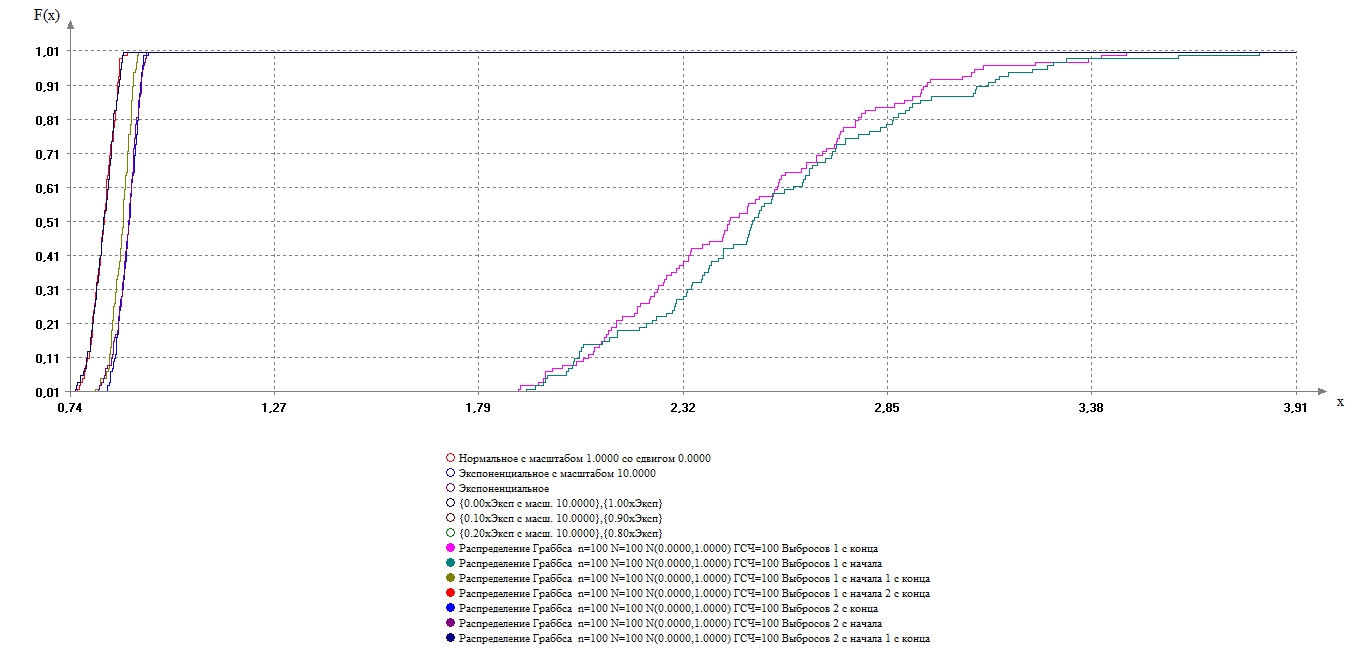
\includegraphics[width=0.75\textwidth]{grabbs}
\caption{Функции распределения статистик критерия типа Граббса при разных
	конфигурациях наблюдений, проверяемых на аномальность.}
\end{figure}

\end{enumerate}

%\section*{Заключение}
%\addcontentsline{toc}{section}{Заключение}

%Заключение.

\section*{Список источников}
\addcontentsline{toc}{section}{Список источников}


1. Статистический анализ данных, моделирование и исследование вероятностных
закономерностей. Компьютерный подход : монография / Б.Ю. Лемешко, С.Б. Лемешко,
\mbox{С.Н. Постовалов}, Е.В Чимитова. --- Новосибирск : Изд-во НГТУ, 2011. --- 888 с.
(серия <<\mbox{Монографии НГТУ}>>).

\end{document}

# vim: ts=2 sw=2
